%%%%%%%%%%%%%%%%%%%%%%%%%%%%%%%%%%%%%%%%%
% Structured General Purpose Assignment
% LaTeX Template
%
% This template has been downloaded from:
% http://www.latextemplates.com
%
% Original author:
% Ted Pavlic (http://www.tedpavlic.com)
%
% Note:
% The \lipsum[#] commands throughout this template generate dummy text
% to fill the template out. These commands should all be removed when
% writing assignment content.
%
%%%%%%%%%%%%%%%%%%%%%%%%%%%%%%%%%%%%%%%%%

%----------------------------------------------------------------------------------------
%	PACKAGES AND OTHER DOCUMENT CONFIGURATIONS
%----------------------------------------------------------------------------------------

\documentclass{article}

\usepackage{fancyhdr} % Required for custom headers
\usepackage{lastpage} % Required to determine the last page for the footer
\usepackage{extramarks} % Required for headers and footers
\usepackage{graphicx} % Required to insert images
\usepackage{lipsum} % Used for inserting dummy 'Lorem ipsum' text into the template
\usepackage{movie15}
\usepackage{hyperref}
\usepackage{amsmath, bm}
\usepackage{listings} 

% Margins
\topmargin=-0.45in
\evensidemargin=0in
\oddsidemargin=0in
\textwidth=6.5in
\textheight=9.0in
\headsep=0.25in

\linespread{1.1} % Line spacing

% Set up the header and footer
\pagestyle{fancy}
\lhead{\hmwkAuthorName} % Top left header
\chead{\hmwkClass\ \hmwkTitle} % Top center header
\rhead{\firstxmark} % Top right header
\lfoot{\lastxmark} % Bottom left footer
\cfoot{} % Bottom center footer
\rfoot{Page\ \thepage\ of\ \pageref{LastPage}} % Bottom right footer
\renewcommand\headrulewidth{0.4pt} % Size of the header rule
\renewcommand\footrulewidth{0.4pt} % Size of the footer rule

\setlength\parindent{0pt} % Removes all indentation from paragraphs

%----------------------------------------------------------------------------------------
%	DOCUMENT STRUCTURE COMMANDS
%	Skip this unless you know what you're doing
%----------------------------------------------------------------------------------------

% Header and footer for when a page split occurs within a problem environment
\newcommand{\enterProblemHeader}[1]{
\nobreak\extramarks{#1}{#1 continued on next page\ldots}\nobreak
\nobreak\extramarks{#1 (continued)}{#1 continued on next page\ldots}\nobreak
}

% Header and footer for when a page split occurs between problem environments
\newcommand{\exitProblemHeader}[1]{
\nobreak\extramarks{#1 (continued)}{#1 continued on next page\ldots}\nobreak
\nobreak\extramarks{#1}{}\nobreak
}

\setcounter{secnumdepth}{0} % Removes default section numbers
\newcounter{homeworkProblemCounter} % Creates a counter to keep track of the number of problems

\newcommand{\homeworkProblemName}{}
\newenvironment{homeworkProblem}[1][Problem \arabic{homeworkProblemCounter}]{ % Makes a new environment called homeworkProblem which takes 1 argument (custom name) but the default is "Problem #"
\stepcounter{homeworkProblemCounter} % Increase counter for number of problems
\renewcommand{\homeworkProblemName}{#1} % Assign \homeworkProblemName the name of the problem
\section{\homeworkProblemName} % Make a section in the document with the custom problem count
\enterProblemHeader{\homeworkProblemName} % Header and footer within the environment
}{
\exitProblemHeader{\homeworkProblemName} % Header and footer after the environment
}

\newcommand{\problemAnswer}[1]{ % Defines the problem answer command with the content as the only argument
\noindent\framebox[\columnwidth][c]{\begin{minipage}{0.98\columnwidth}#1\end{minipage}} % Makes the box around the problem answer and puts the content inside
}

\newcommand{\homeworkSectionName}{}
\newenvironment{homeworkSection}[1]{ % New environment for sections within homework problems, takes 1 argument - the name of the section
\renewcommand{\homeworkSectionName}{#1} % Assign \homeworkSectionName to the name of the section from the environment argument
\subsection{\homeworkSectionName} % Make a subsection with the custom name of the subsection
\enterProblemHeader{\homeworkProblemName\ [\homeworkSectionName]} % Header and footer within the environment
}{
\enterProblemHeader{\homeworkProblemName} % Header and footer after the environment
}

%----------------------------------------------------------------------------------------
%	NAME AND CLASS SECTION
%----------------------------------------------------------------------------------------

\newcommand{\hmwkTitle}{MATLAB Assignment 1} % Assignment title
\newcommand{\hmwkDueDate}{Wednesday, Apr.\ 23,\ 2014} % Due date
\newcommand{\hmwkClass}{EEC\ 263} % Course/class
%\newcommand{\hmwkClassTime}{10:30am} % Class/lecture time
%\newcommand{\hmwkClassInstructor}{Jones} % Teacher/lecturer
\newcommand{\hmwkAuthorName}{Wenhao Wu} % Your name

%----------------------------------------------------------------------------------------
%	TITLE PAGE
%----------------------------------------------------------------------------------------

\title{
\vspace{2in}
\textmd{\textbf{\hmwkClass:\ \hmwkTitle}}\\
\normalsize\vspace{0.1in}\small{Due\ on\ \hmwkDueDate}\\
%\vspace{0.1in}\large{\textit{\hmwkClassInstructor\ \hmwkClassTime}}
\vspace{3in}
}

\author{\textbf{\hmwkAuthorName}}
\date{} % Insert date here if you want it to appear below your name

%----------------------------------------------------------------------------------------

\begin{document}

\maketitle

%----------------------------------------------------------------------------------------
%	TABLE OF CONTENTS
%----------------------------------------------------------------------------------------

%\setcounter{tocdepth}{1} % Uncomment this line if you don't want subsections listed in the ToC

\newpage
\tableofcontents
\newpage

%----------------------------------------------------------------------------------------
%	PROBLEM 1
%----------------------------------------------------------------------------------------

% To have just one problem per page, simply put a \clearpage after each problem

\begin{homeworkProblem}
    \begin{homeworkSection}{\homeworkProblemName:~(a)}
		\begin{align}
			\left(
				\begin{array}{c}
					A_1(z) \\
					A_1^R(z)
				\end{array}
			\right)
			&=
			\left[
				\begin{array}{cc}
					1 & \gamma \\
					\gamma & 1
				\end{array}
			\right]
			\left[
				\begin{array}{cc}
					1 & 0 \\
					0 & z^{-1}
				\end{array}
			\right]
			\left(
				\begin{array}{c}
					1 \\
					1
				\end{array}
			\right) \notag \\
			&=
			\left(
				\begin{array}{c}
					1 + \gamma z^{-1} \\
					\gamma + z^{-1}
				\end{array}
			\right),
		\end{align}
		
		\begin{align}
			\left(
				\begin{array}{c}
					A_2(z) \\
					A_2^R(z)
				\end{array}
			\right)
			&=
			\left[
				\begin{array}{cc}
					1 & 1 \\
					1 & 1
				\end{array}
			\right]
			\left[
				\begin{array}{cc}
					1 & 0 \\
					0 & z^{-1}
				\end{array}
			\right]
			\left(
				\begin{array}{c}
					A_1(z) \\
					A_1^R(z)
				\end{array}
			\right) \notag \\
			&=
			\left(
				\begin{array}{c}
					z^{-2} + 2\gamma z^{-1} + 1 \\
					z^{-2} + 2\gamma z^{-1} + 1
				\end{array}
			\right),
		\end{align}
		therefore $A_2(z)=z^{-2} + 2\gamma z^{-1} + 1$, its two zeros are
		\begin{equation}
			Z_{1,2} = -\gamma \pm \sqrt{\gamma^2-1}.
		\end{equation}
		
    \end{homeworkSection}

    \begin{homeworkSection}{\homeworkProblemName:~(b)}
    	\begin{align}
    		R_Y(k) &= R_X(k) + R_V(k) \notag \\
    		&=\frac{A^2}{2}\cos(2\pi f_0k)+r\delta(k),
    	\end{align}
    	therefore
    	\begin{align}
    		S_Y(e^{j\omega})=\frac{\pi}{2}A^2\sum_{k=-\infty}^{+\infty}
    		\left[\delta(\omega-2\pi f_0+2\pi k) + \delta(\omega+2\pi f_0+2\pi
    		k)\right] + r.
    	\end{align}
    	According to Parseval's theorem, we have
		\begin{align}
			\label{eq:EE2_1}
			E[E^2(t;2)] &=
			\frac{1}{2\pi}\int_{-\pi}^{\pi}\|A_2(e^{j\omega})\|^2S_Y(e^{j\omega})d\omega
			\notag \\
			&=
			\frac{1}{2\pi}\int_{-\pi}^{\pi}\left[4\gamma^2+8\cos(\omega)\gamma+(2\cos(2\omega)+2)\right]S_Y(e^{j\omega})d\omega.
		\end{align}
		Without loss of generality, assuming $0<f_0\leq1/2$, the integration
		in~(\ref{eq:EE2_1}) results in
		\begin{align}
			E[E^2(t;2)] &= (4r + 2A^2)\gamma^2+4A^2\cos(2\pi f_0)\gamma + [2r + A^2 +
			A^2\cos(4\pi f_0)],
		\end{align}
		therefore the optimum reflection coefficient $\gamma$ to minimize the MSE is
		\begin{align}
			\hat{\gamma} = -\frac{\frac{A^2}{2r}\cos(2\pi f_0)}{1 + \frac{A^2}{2r}},
		\end{align}
		and the corresponding MSE is
		\begin{align}
			MSE(2) &= 2r\frac{1 + (1+2\cos^2(2\pi f_0))\frac{A^2}{2r}}
			{1+\frac{A^2}{2r}}.
		\end{align}
		As a result, $\gamma$ can be used to estimate $f_0$ by
		\begin{equation}
			\label{eq:f_0}
			\hat{f}_0=\frac{1}{2\pi}\cos^{-1}\left(-\hat{\gamma}\frac{1+\frac{A^2}{2r}}{\frac{A^2}{2r}}\right),
		\end{equation}
		and when $A^2/2r\rightarrow\infty$, we have
		\begin{align}
			\hat{\gamma} \rightarrow & -\cos(2\pi f_0),\label{eq:f_0_asympt}\\
			MSE(2) \rightarrow & (2+4\cos^2(2\pi f_0))r.
		\end{align}
    \end{homeworkSection}
    
    \begin{homeworkSection}{\homeworkProblemName:~(c)}
		Denote
		\begin{align}
			\mathbf{E}=
			\left(
				\begin{array}{c}
					E(T)\\
					E(T-1)\\
					\cdots\\
					E(2)
				\end{array}
			\right),
		\end{align}
		\begin{align}
			\mathbf{Y}=
			\left[
				\begin{array}{cc}
					2Y(T-1) & Y(T)+Y(T-2)\\
					2Y(T-2) & Y(T-1)+Y(T-3)\\
					\cdots\\
					2Y(1) & Y(2)+Y(0)
				\end{array}
			\right],
		\end{align}
		\begin{align}
			\bm{\gamma}=
			\left(
				\begin{array}{c}
					\gamma \\
					1
				\end{array}
			\right).
		\end{align}
		Then we have
		\begin{align}
			J &= \frac{1}{T-1}\mathbf{E}^T\mathbf{E} \notag \\
			&= \frac{1}{T-1}\bm{\gamma}^T\mathbf{Y}^T\mathbf{Y}\bm{\gamma} \notag\\
			&= \frac{1}{T-1}(a\gamma^2+2b\gamma+c)
		\end{align}
		where
		\begin{align}
			\mathbf{Y}^T\mathbf{Y} &= \left[\begin{array}{cc}a&b\\b&c\end{array}\right]
		\end{align}
		is a positive semi-definite matrix. Then the optimal $\gamma$ to minimize $J$
		is
		\begin{align}
			\hat{\gamma} &= -\frac{b}{a}.
		\end{align}
		Inspired by~(\ref{eq:f_0_asympt}), one simple way to estimate $f_0$ from $\gamma$
    	\begin{align}
    		\hat{f}_0 = \frac{1}{2\pi}\cos^{-1}(-\gamma).
    	\end{align}
    	The rationale here is that this estimator provides a good estimation when
    	the signal to noise ratio is large, while when signal to noise ratio is low
    	any estimator tends to perform poorly anyway. 
    \end{homeworkSection}
    
    \begin{homeworkSection}{\homeworkProblemName:~(d)}
    	{\bf noisin.m}
    	
		\framebox[\textwidth][l]{\lstinputlisting[language=Matlab,breaklines=true]{../Simulation/1/noisin.m}}
		
		\vspace{6pt}
		{\bf conlat.m}
    	
		\framebox[\textwidth][l]{\lstinputlisting[language=Matlab,breaklines=true]{../Simulation/1/conlat.m}}
		
		\vspace{6pt}
		{\bf plotXYEJ.m}
    	
		\framebox[\textwidth][l]{\lstinputlisting[language=Matlab,breaklines=true]{../Simulation/1/plotXYEJ.m}}
		
		\vspace{6pt}
		These functions are called in the script file {\bf Main.m}
		
		\framebox[\textwidth][l]{\lstinputlisting[language=Matlab,breaklines=true]{../Simulation/1/Main.m}}
    	\vspace{6pt}
    	
    	
    	When $A=10$, $f_0=0.25$, $T=20$, $\Phi=0$, $r=1$, the results are shown in
    	Fig.~\ref{fig:1d}.
    	\begin{figure}[!h]
			\centering
			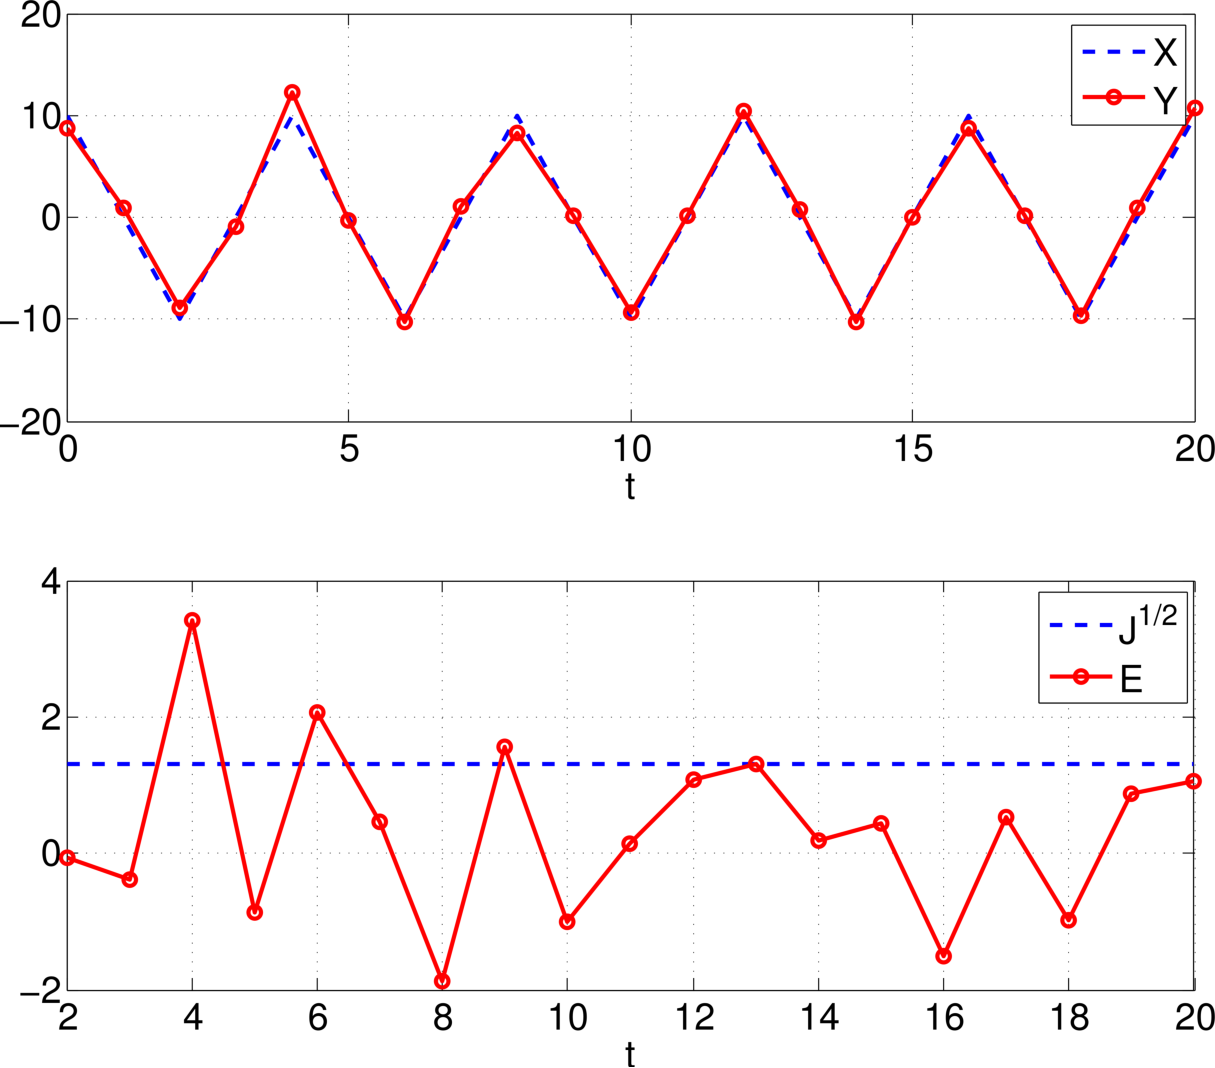
\includegraphics[width=\textwidth]{figs/1d.pdf}
			\caption{$X(t)$, $Y(t)$ and $E(t)$.}
			\label{fig:1d}
		\end{figure}
    	
    \end{homeworkSection}
    \clearpage
    
    \begin{homeworkSection}{\homeworkProblemName:~(e)}
		\begin{enumerate}
		  \item $A=10$, $f_0=0.25$
		  		\begin{table}[h]
					\centering
					\begin{tabular}{c|ccc}
						\hline
						$T$ & $\gamma$ & $J$ & $\hat{f}_0$ \\
						\hline
						10 & -0.018646 & 2.8708 & 0.24703 \\
						20 & 0.006966 & 2.2364 & 0.25111 \\
						50 & -0.0030675 & 2.7354 & 0.24951 \\
						100 & -0.0011253 & 1.4265 & 0.24982 \\
						\hline
					\end{tabular}
				\end{table}
		  \item $f_0=0.05$, $T=100$
		  		\begin{table}[h]
					\centering
					\begin{tabular}{c|ccc}
						\hline
						$A$ & $\gamma$ & $J$ & $\hat{f}_0$ \\
						\hline
						1 & -0.20207 & 3.165 & 0.21762 \\ 
						4 & -0.84035 & 5.0733 & 0.091176\\
						10 & -0.94341 & 2.304 & 0.053799\\
						20 & -0.94852 & 3.9141 & 0.051291\\
						\hline
					\end{tabular}
				\end{table}
		  \item $A=10$, $T=100$
		  		\begin{table}[h]
					\centering
					\begin{tabular}{c|ccc}
						\hline
						$f_0$ & $\gamma$ & $J$ & $\hat{f}_0$ \\
						\hline
						0.01 & -0.97846 & 5.6564 & 0.033095 \\
						0.05 & -0.93032 & 5.3695 & 0.059767 \\
						0.1 & -0.79622 & 3.7875 & 0.10342 \\
						0.25 & 0.0020769 & 2.0953 & 0.25033 \\
						0.5 & 0.98901 & 6.927 & 0.47638 \\
						\hline
					\end{tabular}
				\end{table}
		\end{enumerate}
		It seems that the estimation of $f_0$ becomes more accurate as $T$ and $A$
		grows, while the estimation of $f_0$ is more accurate when $f_0\approx0.25$.
    \end{homeworkSection}
\end{homeworkProblem}
\clearpage

%----------------------------------------------------------------------------------------
%	PROBLEM 2
%----------------------------------------------------------------------------------------

\begin{homeworkProblem}
    \begin{homeworkSection}{\homeworkProblemName:~(a)}
		Denote the tap weight of the desired Wiener filter as
		$\mathbf{a}=[a_0,a_1,\ldots,a_{N-1}]^T$. The normal equation we need to solve
		is
		\begin{align}
			\label{eq:normal}
			\mathbf{K}_Y\mathbf{a}=\mathbf{K}_{YX}
		\end{align}
		where $\mathbf{K}_Y$ is the auto covariance matrix of
		$[Y(t),Y(t-1),\ldots,Y(t-(N-1))]^T$
		\begin{align}
			\mathbf{K}_Y &= 
			\left[
				\begin{array}{cccc}
					1 & a & \cdots & a^{N-1} \\
					a & 1 & \ddots & a^{N-2} \\
					\vdots & \ddots & \ddots & \vdots \\
					a^{N-1} & a^{N-2} & \cdots & 1
				\end{array}
			\right]
			+r\mathbf{I}
		\end{align}
		where $\mathbf{K}_{YX}$ is the cross covariance matrix between
		$[Y(t),Y(t-1),\ldots,Y(t-(N-1))]^T$ and $X(t)$
		\begin{align}
			\mathbf{K}_{YX} &= [1, a,\ldots,a^{N-1}]^T
		\end{align}
		Since $\mathbf{K}_Y$ is central symmetric Toeplitz,~(\ref{eq:normal}) can be
		efficiently solved with Levinson recursion. We design the matlab
		function filterWienerFIR() to design the FIR Wiener filter and return the MSE.
		{\bf filterWienerFIR.m}
    	
		\framebox[\textwidth][l]{\lstinputlisting[language=Matlab,breaklines=true]{../Simulation/2/filterWienerFIR.m}}
    	\vspace{6pt}
    	
    \end{homeworkSection}

    \begin{homeworkSection}{\homeworkProblemName:~(b)}
		When $r = 1$, $a = 0.8$, the MSE and filter tap weights are
    	\begin{table}[h]
			\centering
			\begin{tabular}{c|ccccc}
				\hline
				$N$ & 1 & 2 & 5 & 10 & 20 \\
				\hline
				MSE & 0.5 & 0.40476 & 0.37546 & 0.375 & 0.375 \\
				\hline
				$a_0$ & 0.5000 & 0.4048 & 0.3755 & 0.3750 & 0.3750 \\
				$a_1$ &  & 0.2381 & 0.1883 & 0.1875 & 0.1875 \\
				$a_2$ &  &  & 0.0952 & 0.0938 & 0.0938 \\ 
				$a_3$ &  &  & 0.0498 & 0.0469 & 0.0469 \\
				$a_4$ &  &  & 0.0293 & 0.0234 & 0.0234 \\
				$a_5$ &  &  &  & 0.0117 & 0.0117 \\
				$a_6$ &  &  &  & 0.0059 & 0.0059 \\
				$a_7$ &  &  &  & 0.0030 & 0.0029 \\
				$a_8$ &  &  &  & 0.0016 & 0.0015 \\
				$a_9$ &  &  &  & 0.0009 & 0.0007 \\
				$a_{10}$ &  &  &  &  & 0.0004 \\
				$a_{11}$ &  &  &  &  & 0.0002 \\
				$a_{12}$ &  &  &  &  & 0.0001 \\
				$a_{13}$ &  &  &  &  & 0.0000 \\
				$a_{14}$ &  &  &  &  & 0.0000 \\
				$a_{15}$ &  &  &  &  & 0.0000 \\
				$a_{16}$ &  &  &  &  & 0.0000 \\
				$a_{17}$ &  &  &  &  & 0.0000 \\
				$a_{18}$ &  &  &  &  & 0.0000 \\
				$a_{19}$ &  &  &  &  & 0.0000 \\
				\hline
			\end{tabular}
		\end{table}
		Note that in Example 7.3.2 in the textbook, the causal IIR Wiener filter
		results in a MSE of 0.375, which is approximatedly the same as the FIR filter
		when $N\geq 10$.
    \end{homeworkSection}

    \begin{homeworkSection}{\homeworkProblemName:~(c)}
		When $r=1$, $N=10$, MSE versus a are plotted in Fig.~\ref{fig:2c}. The larger
		$a$ is, i.e.the more $X(t)$ are related to $Y(t),\ldots,Y(t-(N-1))$, the more
		accurate the Wiener filter will be.
		
		\begin{figure}[!h]
			\centering
			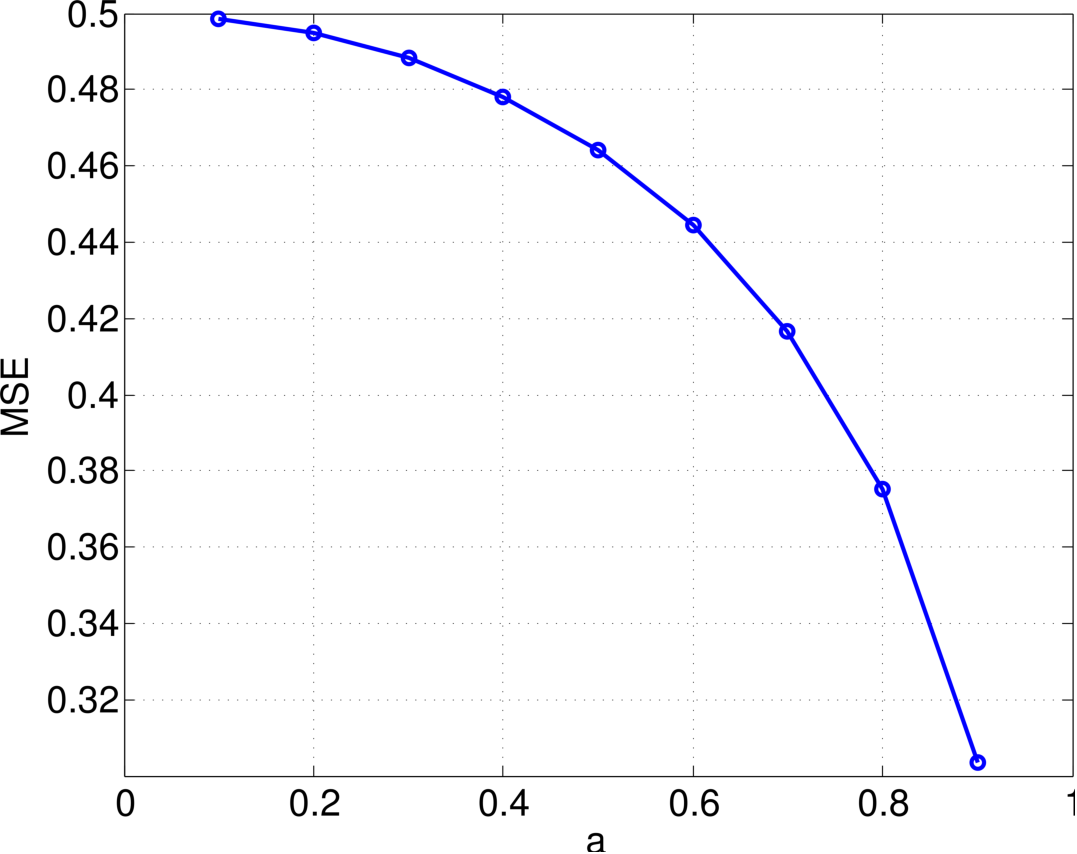
\includegraphics[width=\textwidth]{figs/2c.pdf}
			\caption{MSE versus $a$.}
			\label{fig:2c}
		\end{figure}
    \end{homeworkSection}

\end{homeworkProblem}
\clearpage

%----------------------------------------------------------------------------------------
%	PROBLEM 3
%----------------------------------------------------------------------------------------

\begin{homeworkProblem}
    \begin{homeworkSection}{\homeworkProblemName:~(a)}
    	$X(t)$ and $Y_1(t)$ are shown in Fig.~\ref{fig:3a}.
		\begin{figure}[!h]
			\centering
			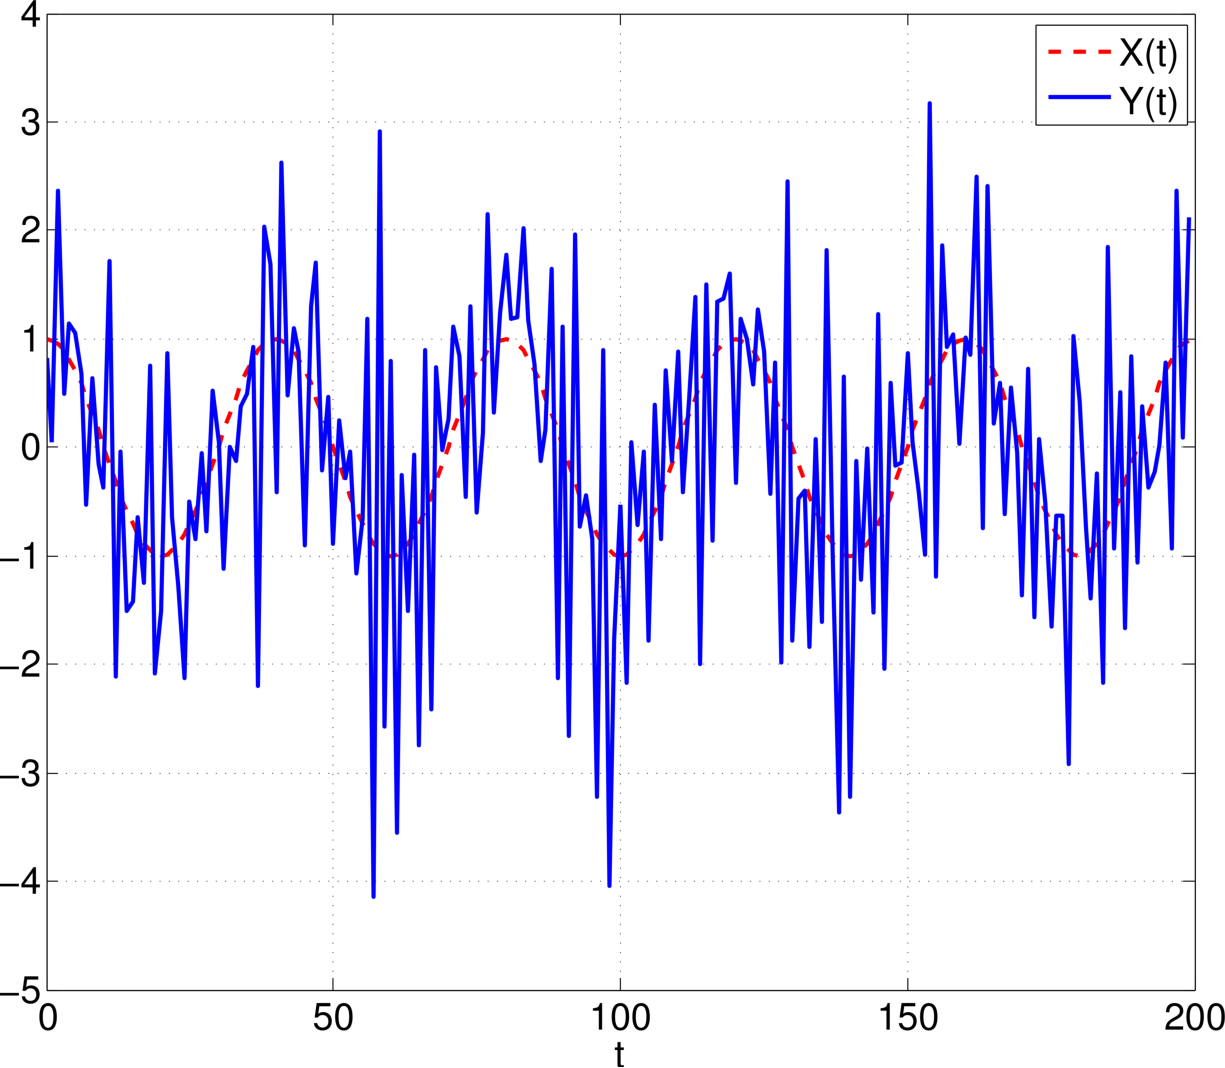
\includegraphics[width=\textwidth]{figs/3a.pdf}
			\caption{$X(t)$ and $Y_1(t)$.}
			\label{fig:3a}
		\end{figure}
    \end{homeworkSection}

    \begin{homeworkSection}{\homeworkProblemName:~(b)}
		Again we use Levinson recursion to get the optimum FIR filter.
		
		{\bf noisin.m}
    	
		\framebox[\textwidth][l]{\lstinputlisting[language=Matlab,breaklines=true]{../Simulation/3/filterWienerFIR.m}}
    \end{homeworkSection}
    
    \begin{homeworkSection}{\homeworkProblemName:~(c)}
		The noise cancellation results are shown in Fig.~\ref{fig:3c1},
		Fig.~\ref{fig:3c2} and Fig.~\ref{fig:3c3}.
		
		\begin{figure}[!h]
			\centering
			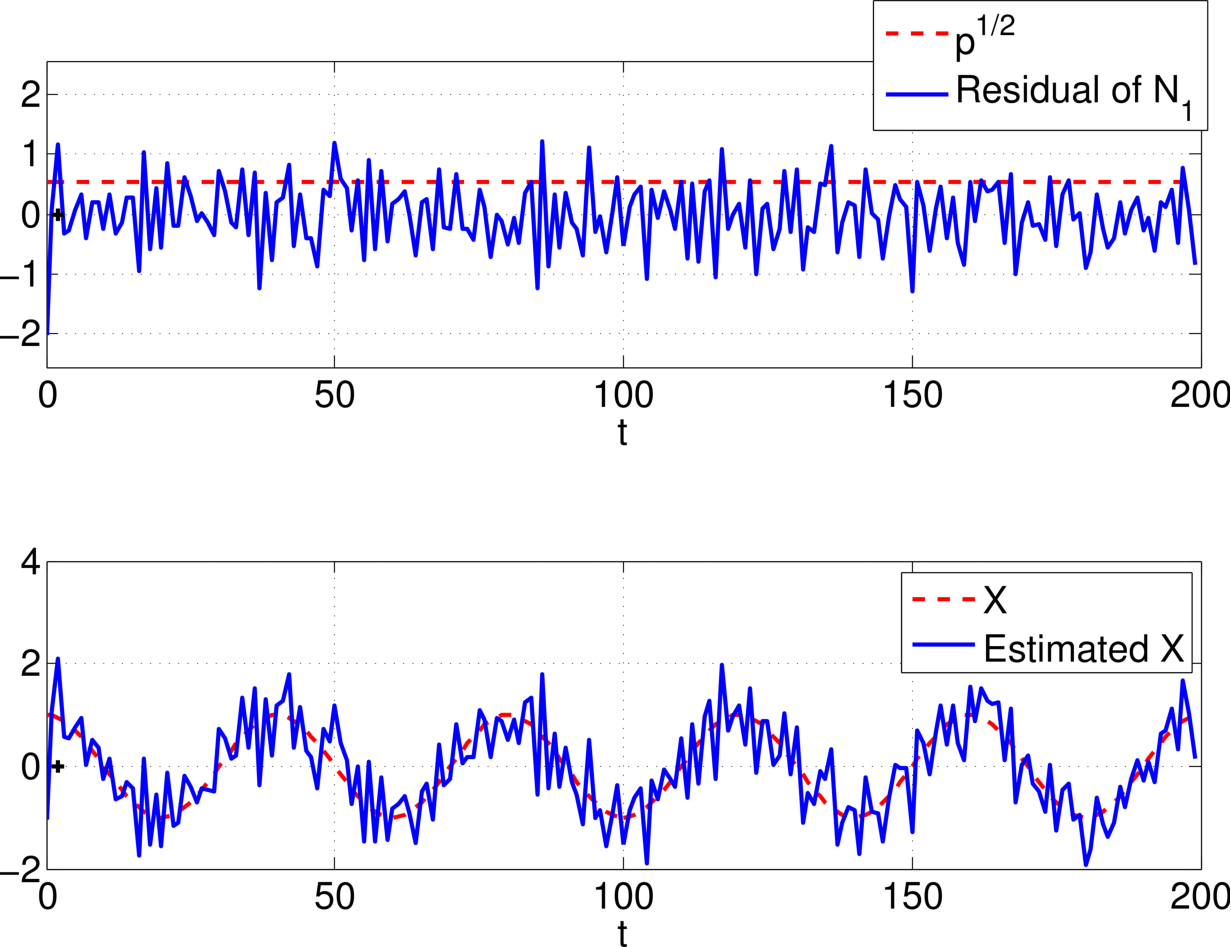
\includegraphics[width=0.5 \textwidth]{figs/3c1.pdf}
			\caption{$M=2$.}
			\label{fig:3c1}
		\end{figure}

		\begin{figure}[!h]
			\centering
			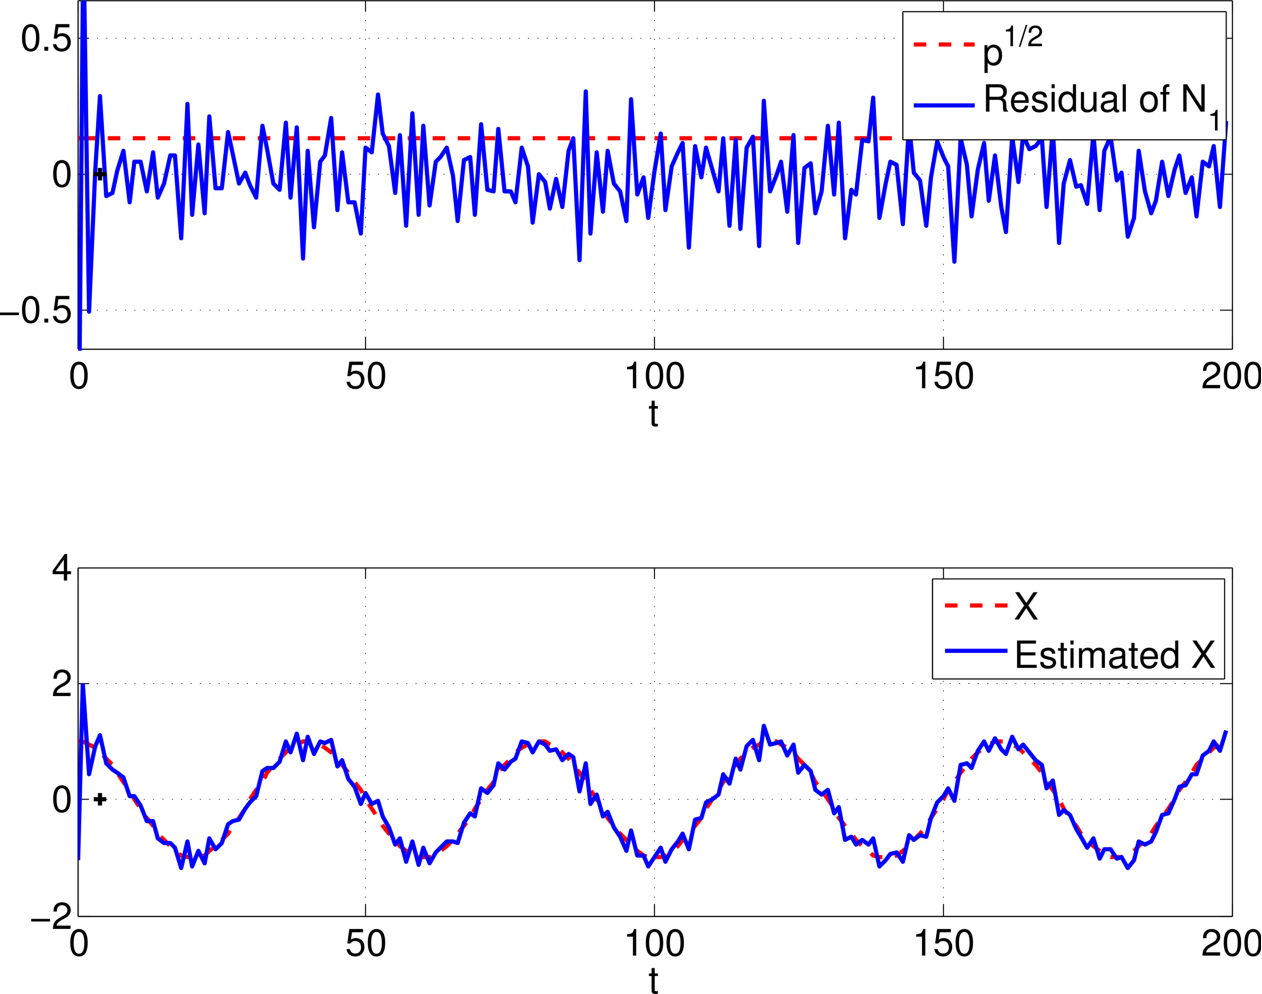
\includegraphics[width=0.5 \textwidth]{figs/3c2.pdf}
			\caption{$M=4$.}
			\label{fig:3c2}
		\end{figure}
		
		\begin{figure}[!h]
			\centering
			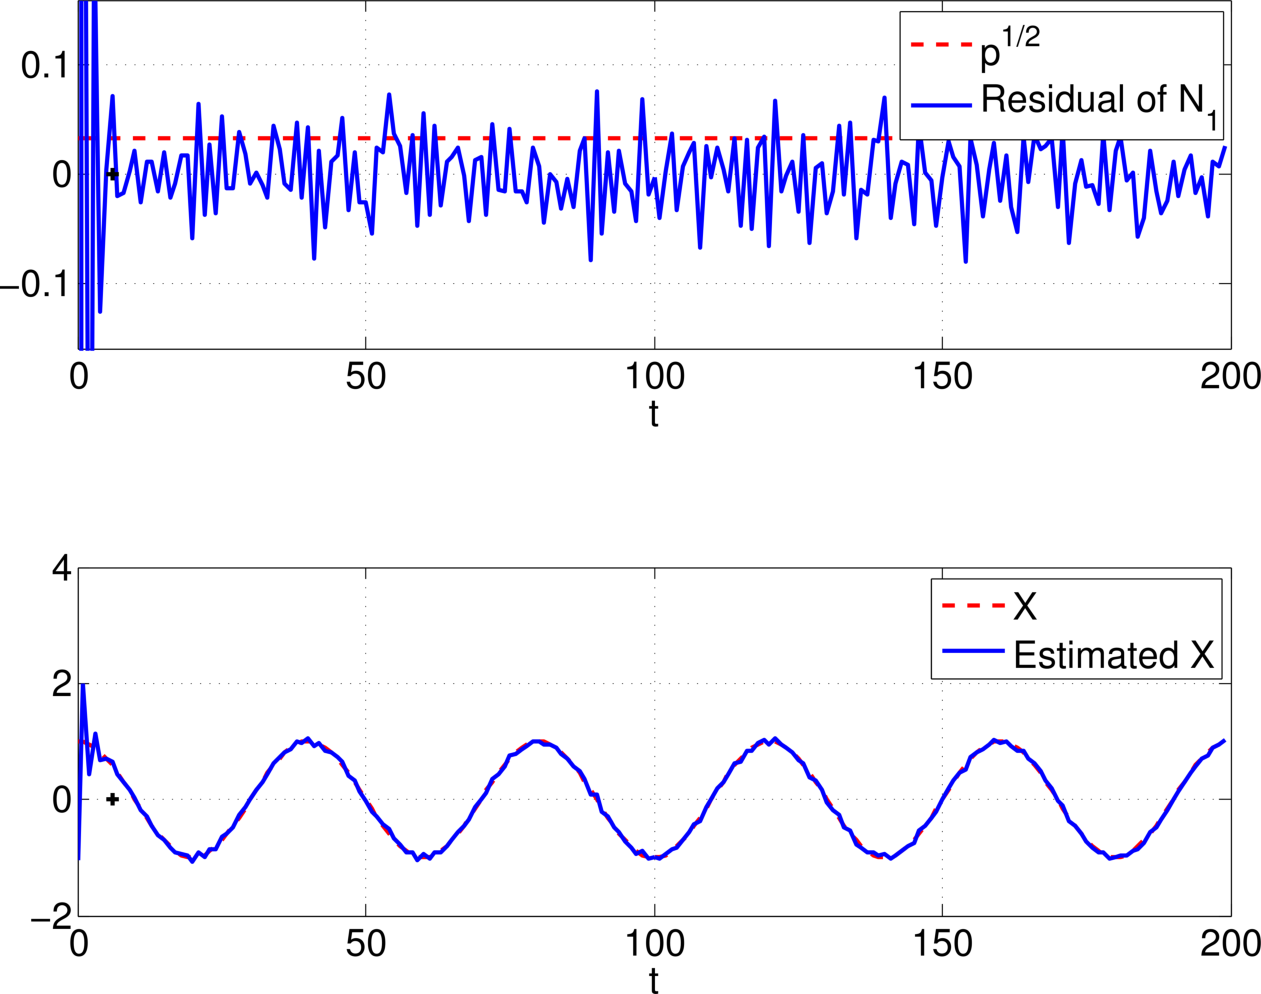
\includegraphics[width=0.5 \textwidth]{figs/3c3.pdf}
			\caption{$M=6$.}
			\label{fig:3c3}
		\end{figure}
    \end{homeworkSection}
    \clearpage
    
    \begin{homeworkSection}{\homeworkProblemName:~(d)}
		In terms of sample MSE, the comparison between the Wiener filter computed with
		theoratical and sampled autocorrelation and cross correlation is shown in
		Table~\ref{table:3d}.
		\begin{table}[h]
			\centering
			\caption{Comparison between the MSE of the Wiener filters evaluated with
		theoratical and sampled autocorrelation and cross correlation.}
			\label{table:3d}
			\begin{tabular}{c|ccc}
				\hline
				$M$ & Theoretical MSE & Sampled MSE(exact correlation) & Sampled 
				MSE(sampled correlation) \\
				\hline
				$2$ & 0.28741 & 0.33904 & 0.33654 \\
				$4$ & 0.017963 & 0.024541 & 0.02542 \\
				$6$ & 0.0011227 & 0.0048859 & 0.0061211 \\ 
				\hline
			\end{tabular}
		\end{table}
    \end{homeworkSection}
    
    \begin{homeworkSection}{\homeworkProblemName:~(e)}
		The sampled MSE results of the Wiener filter evaluated with sampled
		correlation with channel leakage are shown in Table~\ref{table:3e}, whhich
		illustrate that leakage indeed results in an increase in MSE.
		\begin{table}[h]
			\centering
			\caption{Effect of channel leakage on the sampled MSE.}
			\label{table:3e}
			\begin{tabular}{c|ccc}
				\hline
				$M$ & $b=0$ & $b=0.1$ & $b=0.2$ \\
				\hline
				$2$ & 0.29162 & 0.29371 & 0.29613 \\
				$4$ & 0.038405 & 0.040677 & 0.043277 \\
				$6$ & 0.023206 & 0.025529 & 0.028177 \\ 
				\hline
			\end{tabular}
		\end{table}
    \end{homeworkSection}

\end{homeworkProblem}
\clearpage

\end{document}